\mysection{Implementation and Evaluation}
\label{section:evaluation}


We implemented our policy enforcement mechanism atop a Freescale i.MX53 Quick
Start Board as our guest device. This TrustZone-enabled board has a 1GHz ARM
Cortex A8 processor with 1GB DDR3 RAM. We chose this board as the guest device
because it offers open, programmable access to the secure world. In contrast,
the vendors of most commercially-available TrustZone-enabled devices today lock
down the secure world and prevent any modifications to it. A small part of main
memory is reserved for exclusive use by the secure world. On our i.MX53 board,
we assigned the secure world 256MB of memory, although it may be possible to
reduce this with future optimizations. The normal world runs Android 2.3.4 atop
Linux kernel version 2.6.35.3.


%\begin{wrapfigure}{lt}{1.5in}
\begin{figure}[t!]
\footnotesize
\renewcommand{\arraystretch}{0.75}
\centering
%\indent\vspace{-0.5cm}
\begin{tabular}{|l|r|}
\hline
\multicolumn{1}{|c|}{\bf Component Name} & \multicolumn{1}{|c|}{\bf LOC}\\
\hline
\hline
\multicolumn{2}{|c|}{\bf Secure World (TCB)}\\
\hline
(1) Memory manager            & 1,381\\
(2) Authentication            & 1,285\\
(3) Memory ops                & 305\\
\hline
(4) SHA1+HMAC                 & 861\\
(5) X509                      & 877\\
(6) RSA                       & 2,307\\
\hline
\hline
\multicolumn{2}{|c|}{\bf Normal World}\\
\hline
(1) Kernel module             & 93\\
(2) UI app                    & 72\\
\hline
\end{tabular}
%\indent\vspace{-0.3cm}
\mycaption{Sizes of components executing on the guest.}
{\label{table:loc}}
%\indent\vspace{-0.45cm}
\end{figure}
%\end{wrapfigure}
%
We built a bare-metal runtime environment for the secure world, just enough to
support the components shown in \figref{figure:overall}. This environment has a
memory manager, and a handler to parse and process commands received from the
host via the normal world. To implement cryptographic operations, we used
components from an off-the-shelf library called PolarSSL
(v1.3.9)~\cite{polarssl}. Excluding the cryptography library, our TCB in the
secure world consists of about 3,000 lines of C code, including about 250 lines
of inline assembly.  


\figref{table:loc} shows the sizes of various components.  We used PolarSSL's
implementation of SHA1 and HMACs, RSA and X509 certificates.  As shown in
\figref{table:loc}, the files implementing these components alone comprise only
about 4,000 lines of code. In addition to these TCB components, we built the
kernel module and the UI app (written as a native daemon) for the normal world,
comprising 165 lines of code.  We implemented a host policy server that
authenticates guest devices, and performs remote memory operations.  We
conducted experiments to showcase the utility of remote reads and writes to
enforce the host's policies on the guest. The guest and the host communicate
over WiFi.

%
% PolarSSL consists of about 73,000 lines of C code and dominates our TCB.
% However, our implementation only uses a limited subset of the functionality
% in PolarSSL (SHA1 and HMACs, RSA and X509 certificates).  Together with their
% dependencies, we estimate a stripped-down version of PolarSSL supporting just
% the required functionality would be approximately 9,000 lines of code.
% However, we have not attempted to create such a stripped-down library.

% Server: 1756 (plus 48LOC of python for memory analysis). Not really
% important, so we won't report this. 

\myparagraph{Guest Device Analysis}
%
To illustrate the power of remote memory read operations to perform device
analysis, we wrote a simple rootkit that infects the guest's normal world
kernel by hooking its system call table. In particular, it replaces the entry
for the \texttt{close} system call to instead point to a malicious function
injected into the kernel. The malicious functionality ensures that if the
process invoking \texttt{close} calls it with a magic number, then the process
is elevated to \texttt{root}.  Although simple in its operation, Petroni and
Hicks~\cite{sbcfi:ccs07} show that over 95\% of all rootkits that modify kernel
data operate this way.

We were able to detect this rootkit on the host by remotely reading and
analyzing the guest's memory pages. We remotely read pages containing the
\texttt{init}, \texttt{text} and \texttt{data} sections of kernel memory. Our
analyzer, a 48 line Python script, reads the addresses in the system call table
from memory, and compares these entries with addresses in \texttt{System.map}.
If the address is not included, \eg~as happens if the entry for the
\texttt{close} system call is modified, it raises an error. Prior work
(\eg~\cite{sbcfi:ccs07,gib:tdsc11,kop:ccs09}) has developed tools to
recursively traverse kernel data structures from memory dumps. Such tools can
also be used with the memory pages obtained by the host to detect more
sophisticated rootkits.

For the above experiment, it took the secure world 54 seconds to create an HMAC
over the memory pages that were sent to the host (9.2MB in total). It takes
under a second to copy data from the normal world to the secure world and vice
versa. It may be possible to accelerate the performance of the HMAC
implementation using floating point registers and hardware acceleration, but we
have not done so in our prototype.


\myparagraph{Guest Device Control}
%
We evaluated the host's ability to dynamically reconfigure a guest device via
remote memory write operations. For this experiment, we attempted to disable a
number of peripherals from the guest device. However, the i.MX53 board only
supports a bare-minimum number of peripherals. As proof-of-concept, we
therefore tested the effectiveness of remote writes on a Samsung Galaxy Nexus
smart phone with a Texas Instruments OMAP 4460 chipset. This chipset has a
1.2GHz dual-core ARM Cortex-A9 processor with 1GB of RAM, and runs Android 4.3
atop Linux kernel version 3.0.72. This device has a rich set of peripherals,
but its chipset comes with TrustZone locked down, \ie~the secure world is not
accessible to third-party programmers.  We therefore performed remote writes by
modifying memory using a kernel module in its (normal world) operating system.
Thus, while remote writes to this device do not enjoy the security properties
described in \sectref{section:mechanism}, they allow us to evaluate the ability
to uninstall a variety of peripherals from a running guest device.

\begin{figure}[t!]
\centering
\footnotesize
\begin{tabular}{cc}
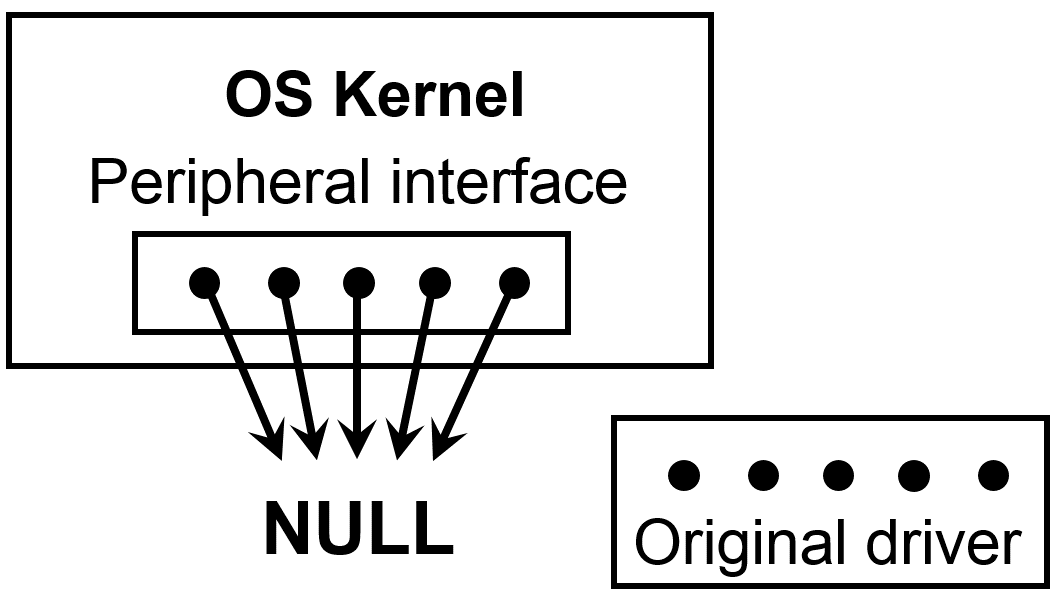
\includegraphics[keepaspectratio=true,height=0.85in]{figures/driver-null.png} & 
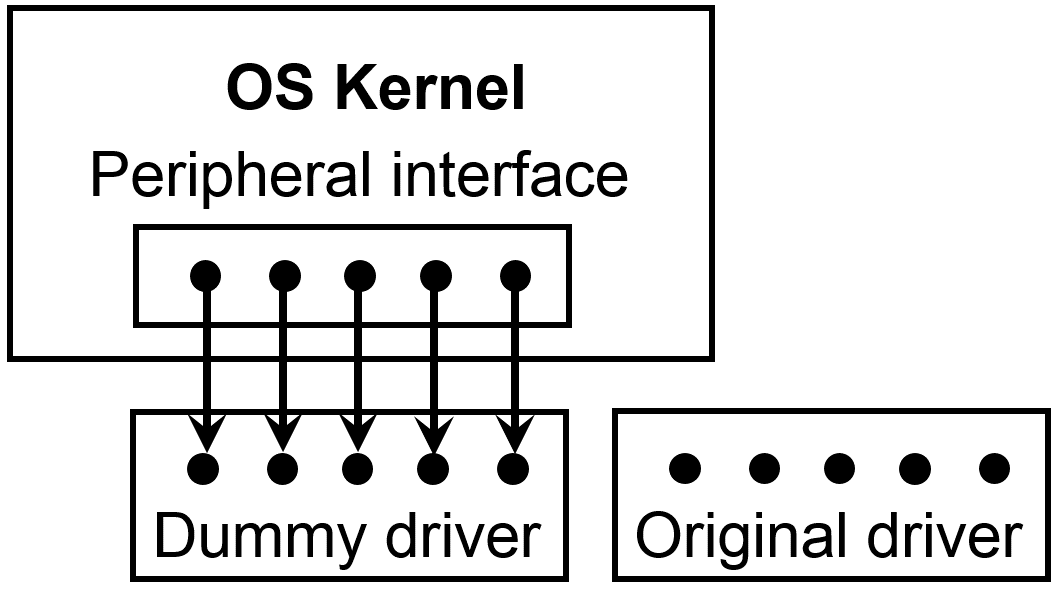
\includegraphics[keepaspectratio=true,height=0.85in]{figures/driver-dummy.png}\\
\textbf{(a)~\textsc{null}ifying the interface} &
\textbf{(b)~Installing a dummy driver}\\
\end{tabular}
%\indent\vspace{-0.3cm}
\mycaption{Uninstalling a peripheral by writing to kernel memory. Each device
driver exposes an interface and is linked to the kernel via function pointers.
%Part~(a) shows how peripheral device drivers are linked to the kernel.
Part~(a) shows how to uninstall the peripheral by making the kernel's device 
interface point to \textsc{null} bytes.
Part~(b) shows how to uninstall the peripheral by unlinking the original driver
and instead linking a dummy driver.}
{\label{figure:uninstall}}
%\indent\vspace{-0.4cm}
\end{figure}

We adopted two broad strategies to uninstall peripherals. On modern operating
systems, each peripheral has an interface within the kernel.  This interface
consists of a set of function pointers that are normally set to point to the
corresponding functions within the peripheral's device driver, which
communicates with the peripheral. 


\begin{figure}[t!]
\footnotesize
\centering
\renewcommand{\arraystretch}{0.75}
\begin{tabular}{|c|c|c|c|}
\hline
\textbf{Peripheral} 
  & \textbf{Method Used} 
  & \textbf{Size (bytes)} 
  & \textbf{Device}\\
\hline
USB (webcam) & \textsc{null}ify interface & 104 & i.MX53\\
USB (webcam) & Dummy driver               & 302 & i.MX53\\
Camera       & \textsc{null}ify interface & 140 & Nexus\\
Camera       & Dummy driver               & 212 & Nexus\\
WiFi         & Dummy driver               & 338 & Nexus\\
3G (Data)    & Dummy driver               & 252 & Nexus\\
3G (Voice)   & Dummy driver               & 224 & Nexus\\
Microphone   & Dummy driver               & 184 & Nexus\\
Bluetooth    & Dummy driver               & 132 & Nexus\\
\hline
\end{tabular}
%\indent\vspace{-0.25cm}
\mycaption{Peripherals uninstalled using remote write operations to a guest
device. Also shown are the method used to uninstall the peripheral (see
\figref{figure:uninstall}), the number of bytes modified or added by the remote
write, and the guest device used.}
{\label{table:uninstall}}
%\indent\vspace{-0.4cm}
\end{figure}

Our first strategy to uninstall the peripheral was to simply set the function
pointers in the peripheral's interface to \textsc{null}, as shown in
\figref{figure:uninstall}(a). If the kernel checks these pointers prior to
invoking the functions, it will simply return an error code to the application
saying that the device is not installed. This approach has the advantage of
only involving simple writes to the kernel (\textsc{null} bytes to certain
addresses), which can easily be validated as safe if the guest so wishes.
However, we found that this approach generally makes the guest unstable. For
example, except in two cases, \textsc{null}ifying the peripheral interface
resulted in a system crash (\figref{table:uninstall}).

\newcommand{\apperr}{\textsc{AppErrMsg}}
\newcommand{\lostconn}{\textsc{LostConn}}
\newcommand{\anderr}{\textsc{AndroidErrMsg}}
\newcommand{\emptyfile}{\textsc{EmptyFile}}
\newcommand{\blnkscrn}{\textsc{BlankScreen}}
\newcommand{\im}{\it\bfseries}

\begin{figure*}[htbp!]
\footnotesize
\begin{center}
%
%\begin{tabular}{|c|p{0.16\textwidth}|p{0.16\textwidth}|p{0.16\textwidth}|p{0.16\textwidth}|p{0.16\textwidth}|}
\begin{tabular}{|c|c|c|c|c|c|}
\hline
{\bf USB} & {\im MobileWebCam} & {\im Camera ZOOM FX} & {\im Retrica} & {\im Candy Camera} & {\im HD Camera Ultra}\\ 
\hline
\textit{Passive}    & \apperr      & \apperr        & \anderr & \apperr      & \anderr\\
\textit{Active}     & \apperr      & \apperr        & \apperr & \apperr      & \apperr\\
\hline
\hline
{\bf Camera} & {\im Camera for Android} & {\im Camera MX} & {\im Camera ZOOM FX} & {\im HD Camera for Android} & {\im HD Camera Ultra} \\
\hline
\textit{Passive}       & \anderr            & \apperr   & \apperr        & \anderr               & \anderr\\
\textit{Active}        & \blnkscrn          & \apperr   & \anderr        & \blnkscrn             & \blnkscrn\\
\hline
\hline
{\bf WiFi} & {\im Spotify} & {\im Play Store} & {\im YouTube} & {\im Chrome Browser} & {\im Facebook}\\
\hline
\textit{Passive} & \lostconn & \lostconn & \lostconn & \lostconn & \lostconn\\
\textit{Active}  & \lostconn & \lostconn & \lostconn & \lostconn & \lostconn\\
\hline
\hline
{\bf 3G (Data)} & {\im Spotify} & {\im Play Store} & {\im YouTube} & {\im Chrome Browser} & {\im Facebook}\\
\hline
\textit{Passive} & \lostconn & \lostconn & \lostconn & \lostconn & \lostconn\\
\textit{Active}  & \lostconn & \lostconn & \lostconn & \lostconn & \lostconn\\
\hline
\hline
{\bf 3G (Voice)} & \multicolumn{5}{c|}{\im Default call application}\\
\hline
\textit{Passive} & \multicolumn{5}{c|}{\apperr: Unable to place a call}\\
\textit{Active}  & \multicolumn{5}{c|}{\apperr: Unable to place a call}\\
% {\bf 3G (Voice)} & \multicolumn{5}{p{0.8\textwidth}|}{\im Default call application}\\
% \hline
% \textit{Passive} & \multicolumn{5}{p{0.8\textwidth}|}{\apperr: Unable to place a call}\\
% \textit{Active}  & \multicolumn{5}{p{0.8\textwidth}|}{\apperr: Unable to place a call}\\
\hline
\hline
{\bf Microphone} & {\im Audio Recorder} & {\im Easy Voice Recorder} & {\im Smart Voice Recorder} & {\im Sound and Voice Recorder} & {\im Voice Recorder}\\
\hline
\textit{Passive}           & \apperr        & \apperr             & \apperr              & \apperr    & \apperr\\
\textit{Active}            & \emptyfile     & \emptyfile          & \emptyfile           & \emptyfile & \emptyfile\\
\hline
\end{tabular}
\end{center}
%
\indent\vspace{-0.75cm}
\mycaption{Results of robustness experiments for both the passive and active
settings.  We use \textit{Passive} to  denote experiments in which the user app
was not running when the peripheral's driver was replaced with a dummy, and the
app was started after this replacement. We use \textit{Active} to denote
experiments in which the periperhal's driver was replaced with a dummy even as
the client app was executing. (1)~\apperr\ denotes the situation where the user
app starts normally, but an error message box is displayed within the app after
it starts up; (2)~\blnkscrn\ denotes a situation where the user app displayed a
blank screen; (3)~\lostconn\ denotes a situation where the user app loses
network connection; (4)~\emptyfile\ denotes a sitution where no error message
is displayed, but the sound file that is created is empty; (5) \anderr\ denotes
the situation where the user app fails to start (in the passive setting) or a
running app crashes (in the active setting), and the Android runtime system
displays an error.}{\label{table:robustness}}
\indent\vspace{-0.65cm}
%
\end{figure*}



We therefore adopted the approach shown in \figref{figure:uninstall}(b), which
should work with any peripheral. In this approach, we write a dummy driver for
the peripheral, \eg~one that simply returns a suitable error code rather than
communicating with the peripheral, and link it with the kernel in place of the
original driver.  With this approach we were successfully able to uninstall all
the peripherals that we tried.  Note that the host must introduce new code
(\ie~the dummy driver) into the guest, so the guests must check the remote
write operations for safety. \sectref{section:vetting} discusses our prototype
vetting service.

\figref{table:uninstall} shows the set of peripherals that we uninstalled, the
method used to uninstall the peripheral, the size of the write operation (the
number of bytes that we had to modify/introduce in the kernel), and whether the
operation was performed on the i.MX53 or the Nexus. We were able to uninstall
the USB on the i.MX53 and the camera on the phone by \textsc{null}ifying the
peripheral interface. For the other peripherals, we introduced dummy drivers.
We also used dummy drivers for the USB and the camera to compare the size of
the write operations. In this case, the size of the write includes both the
bytes modified in the peripheral interface and the dummy driver functions. For
the 3G interface, we considered two cases: that of disabling only data
transmission and that of only disabling calls. Our experiment shows it is
possible to uninstall peripherals without crashing the operating system by just
modifying a few hundred bytes of memory on the running device. 


Installing a dummy driver disables the peripheral, but how does it affect the
user app that is using the peripheral? To answer this question, we conducted
two sets of experiments involving a number of client user apps that leverage
the periperhals shown in \figref{table:uninstall}. 

In the first set of experiments, which we call the \textit{passive setting}, we
start with a configuration where the client app is not executing, replace the
device driver of the peripheral with a dummy, and then start the app. In the
second set of experiments, called the \textit{active setting}, we replace the
periperhal's device driver with the dummy as the client app that uses the
peripheral is executing. 

\figref{table:robustness} shows the results of our experiments. For both the
passive and active settings, we observe that in most cases, the user app
displays a suitable error message or changes its behavior by displaying a blank
screen or creating an empty audio file. In some cases, particularly in the
passive setting, the app fails to start when the driver is replaced, and the
Android runtime displays an error that it is unable to start the app.

